\documentclass[
    ref=bibs/references.bib,
    print,
    colorlinks, % 超链接是否彩色, 不开启时为黑色无边框
    % bibBackref, % 是否在参考文献列表中显示文献引用页, 不开启时为不显示
    % draft, % 指定为草稿模式, 会进行简化使生成更快, 在断行不良/溢出出加黑色方块给出提示
]{styles/ucasDissertation}
\addbibresource{bibs/references.bib}
\graphicspath{{assets}}

\GlsXtrLoadResources[
    src={bibs/symbols.bib, bibs/abbreviations.bib}, % 这里的文件名对应cls文件中创建的术语表名
    type={same as base}, % 设置类型为bib文件名
    sort={letter-case}, % sort according to character code
    symbol-sort-fallback={name},
]

\begin{document}
% ------------------------------------------------------------------------------
% 封面
% \title{随便找了一个有下标的专业名词CsV\textsubscript{3}Sb\textsubscript{5}然后说点废话展示一\\下标题过长怎么处理}{A long title including a term with subscript CsV\textsubscript{3}Sb\textsubscript{5} to indicate\\ how to solve the overflow when the title is too long}
\header{随便找了一个有下标的专业名词CsV\textsubscript{3}Sb\textsubscript{5}然后说点废话展示一下标题过长怎么处理}{A long title including a term with subscript CsV\textsubscript{3}Sb\textsubscript{5} to indicate how to solve the overflow when the title too long}
\degree{硕士} % 硕士/博士
\author{张三}{Zhang San}
\supervisor{李四~教授}{Professor Li Si}{中国科学院大学XX研究所}
\degreeType{电子信息工程}{Master of Electronic and Information Engineering}
\subject{信号与信息处理}{Signal and information processing}
\institute{中国科学院大学YY研究所}{YY Institute of ZZ,\\University of Chinese Academy of Sciences}
\date{2023年~6~月}{June 2023}
\makeCover
% 变量由ucasInfo.sty中提供

\title{
    随便找了一个有下标的专业名词CsV\textsubscript{3}Sb\textsubscript{5}然后说点废话展示一下标题过长会怎么样
}{
    A long title including a term with subscript CsV\textsubscript{3}Sb\textsubscript{5} to indicate what will happens when the title is too long
}
\degree{硕士} % 硕士/博士
\author{张三}{Zhang San}
\supervisor{李四~教授}{Professor Li Si}{中国科学院大学XX研究所}
\degreeType{电子信息工程}{Master of Electronic and Information Engineering}
\subject{信号与信息处理}{Signal and information processing}
\institute{中国科学院大学YY研究所}{YY Institute of ZZ,\\University of Chinese Academy of Sciences}
\gradYear{2023}
% 夏季毕业填6月,冬季毕业填12月
\gradMonth{6}{June}
\makeCover
% 原创性声明及授权使用声明
\makeDeclaration
\frontmatter
% 摘要
\abstract{
这是一段摘要, 摘要摘要摘要摘要摘要摘要摘要摘要摘要摘要摘要摘要摘要摘要摘要摘要摘
要摘要摘要摘要摘要摘要摘要摘要摘要摘要摘要摘要摘要摘要摘要摘要摘要摘要摘要摘要摘
要摘要摘要摘要摘要摘要摘要摘要摘要摘要摘要摘要摘要摘要摘要摘要摘要摘要摘要摘要摘
要摘要摘要.

注意关键词应有3\~{}5个。
}{
This is a abstract, abstract abstract! abstract? abstract, abstract abstrac.
}
\keywords{
关键词1, 关键词2, 关键词3, 关键词4, 关键词5
}{
keyword1, keyword2, keyword3, keyword4, keyword5
}
\makeAbstract
% 目录
\tableofcontents
% 图表目录
\listofmaterials[
    table,
    figure,
    algorithm,
    code,
]
% 符号说明 (术语表)
\listofnotaions
% ------------------------------------------------------------------------------
\mainmatter
\chapter{撰写规范指导意见摘抄}

\section{组成及要求}

\subsection{正文}

正文一般包括绪论、论文主体、研究结论与展望等部分。

\subsubsection{绪论}

绪论应包括选题的背景和意义,国内外相关研究成果与进展述评,本论文所要解决的科学与技术问题、所运用的主要理论和方法、基本思路和论文结构等。绪论应独立成章,用足够的文字叙述,不与摘要雷同。要实事求是,不夸大也不弱化前人的工作和自己的工作。

\subsubsection{论文主体}

论文主体是正文的核心部分,占主要篇幅,它是将学习和研究过程中调查、观察和测试所获得的材料和数据,经过思考判断、加工整理和分析研究,进而形成论点。依据学科专业及具体选题,论文主体可以有不同的表现形式,可以按照章与节的结构表述,也可以按照“研究背景与意义—研究方法与过程—研究结果与讨论”的表述形式组织论文。但主体内容必须实事求是,客观诚实,准确完备,合乎逻辑,层次分明,简明可读。

\subsubsection{研究结论与展望}

研究结论是对整个论文主要成果的总结,不是正文中各章小结的简单重复,应准确、完整、明确、精炼。应明确凝练出本研究的主要创新点,对论文的学术价值和应用价值等加以分析和评价,说明本项研究的局限性或研究中尚难解决的问题,并提出今后进一步在本研究方向进行研究工作的设想或建议。结论部分应严格区分本人研究成果与他人科研成果的界限。

\subsection{参考文献}

本着严谨求实的科学态度撰写论文,凡学位论文中有引用或参考、借鉴他人思想或成果之处,均应按一定的引用规范,列于文末(通篇正文之后),参考文献部分应与正文的文献引用一一对应,注重合理引用,严禁抄袭剽窃等学术不端行为。

\subsection{附录 (若有)}

主要列入正文内过分冗长的公式推导、供查读方便所需的辅助性数学工具或表格、数据图表、程序全文及说明、调查问卷、实验说明等。

\subsection{致谢}

对给予各类资助、指导和协助完成研究工作,以及提供各种对论文工作有利条件的单位及个人表示感谢。致谢应实事求是,切忌浮夸与庸俗之词。致谢末尾应具日期,日期与论文封面一致。

\subsection{作者简历及攻读学位期间发表的学术论文与其他相关学术成果}

作者简历应包括从大学起到申请学位时的个人学习工作经历。按学术论文发表的时间顺序,列出作者本人在攻读学位期间发表或已录用的学术论文清单(著录格式同参考文献)。其他相关学术成果可以是申请的专利、获得的奖项及完成的项目等代表本人学术成就的各类成果。

\section{撰写要求}

\subsection{论文正文}
\subsubsection{图标等编号}

论文中的图、表、附注、公式、算式等,一律用阿拉伯数字分章依序连续编码。其标注形式
应便于互相区别,如:图1-1(第1章第一个图)、图2-2(第2章第二个图);表3-2(第3章
第二个表)等。附录的图表参考正文的编号方式,如附图1-1或附表1-1。

\subsubsection{图和表}

论文中若有图和表,应设置图表目录,先列图后列表,置于目录页后,另页编排。

图片大小适当,图边界在页面范围内(图边界离页面边界距离大于页边距)。若图片中包含
文字,文字大小不超过正文文字大小。\\
图包括曲线图、构造图、示意图、框图、流程图、记录图、地图、照片等,宜插入正文适当
位置。引用的图必须注明来源。具体要求如下:
\begin{enumerate}
    \item 图应具有“自明性”,即只看图、图题和图注,不阅读正文,就可理解图意。每一图应有简短确切的图题,连同图序置于图下居中。
    \item 图中的符号标记、代码及实验条件等,可用最简练的文字横排于图框内或图框外的某一部位作为图注说明,全文统一。图题建议用中文及英文两种文字表达。
    \item 照片图要求主要显示部分的轮廓鲜明,便于制版,如用放大、缩小的复制品,必须清晰,反差适中,照片上应有表示目的物尺寸的标尺。
\end{enumerate}

\chapter{撰写要求}

\section{论文正文}
\subsection{图标等编号}

论文中的图、表、附注、公式、算式等,一律用阿拉伯数字分章依序连续编码。其标注形式
应便于互相区别,如:图1-1(第1章第一个图)、图2-2(第2章第二个图);表3-2(第3章
第二个表)等。附录的图表参考正文的编号方式,如附图1-1或附表1-1。

\subsection{图和表}

论文中若有图和表,应设置图表目录,先列图后列表,置于目录页后,另页编排。

\subsubsection{图}

图片大小适当,图边界在页面范围内(图边界离页面边界距离大于页边距)。若图片中包含
文字,文字大小不超过正文文字大小。\\
图包括曲线图、构造图、示意图、框图、流程图、记录图、地图、照片等,宜插入正文适当
位置。引用的图必须注明来源。具体要求如下:
\begin{itemize}
    \item 图应具有“自明性”,即只看图、图题和图注,不阅读正文,就可理解图意。每一图应有简短确切的图题,连同图序置于图下居中。
    \item 图中的符号标记、代码及实验条件等,可用最简练的文字横排于图框内或图框外的某一部位作为图注说明,全文统一。图题建议用中文及英文两种文字表达。
    \item 照片图要求主要显示部分的轮廓鲜明,便于制版,如用放大、缩小的复制品,必须清晰,反差适中,照片上应有表示目的物尺寸的标尺。
\end{itemize}

\section{功能介绍}

\subsection{数学公式}

比如\autoref{eq:1}
\begin{equation}
    \label{eq:1}
    \int_{-\infty}^{+\infty} e^{-x^2} dx = \sqrt{\pi}
\end{equation}

\subsection{图片}

比如\autoref{fig:pngtest}. 注意模板中已经默认设置figure及table环境的位置参数为\verb|htbp|, 不能再单独设置.
\begin{figure}
    \centering
    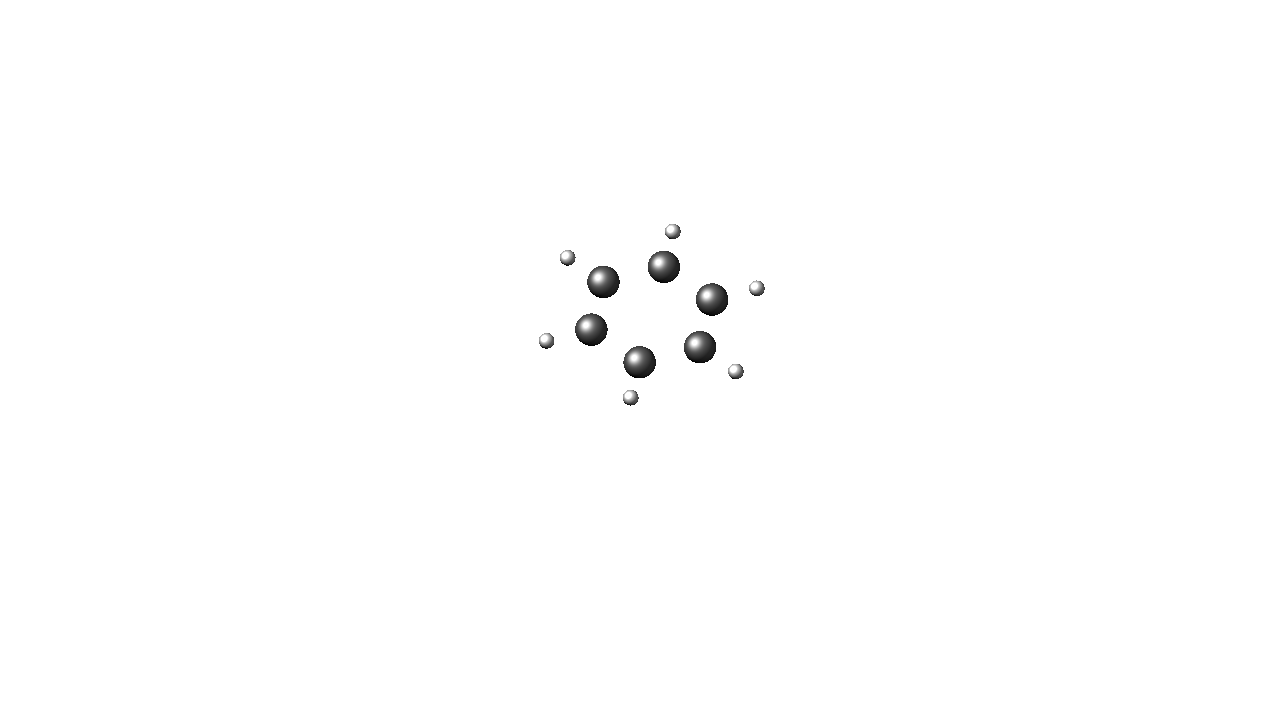
\includegraphics[width=0.5\textwidth]{pngtest}
    \bicaption{ucasthesis 图片测试}{ucasthesis figure test}\label{fig:pngtest}
\end{figure}

\subsection{表格}

请见\autoref{tab:sample}。
\begin{table}
    \bicaption{这是一个样表}{This is a sample table}\label{tab:sample}
    \centering
    \setlength{\tabcolsep}{4pt}% column separation
    \renewcommand{\arraystretch}{1.2}%row space
    \begin{tabular}{lcccccccc}
        \toprule
        行号 & \multicolumn{8}{c}{跨多列的标题}\\
        %\cline{2-9}% partial hline from column i to column j
        \midrule
        Row 1 & 1 & 2 & 3 & 6 & 7 & 8 \\
        Row 2 & 1 & 2 & 3 & 6 & 7 & 8 \\
        Row 3 & 1 & 2 & 3 & 6 & 7 & 8 \\
        Row 4 & 1 & 2 & 3 & 6 & 7 & 8 \\
        \bottomrule
    \end{tabular}
\end{table}

\subsection{术语}

有符号: \gls{pi}, 有缩写: \gls{spi}, 都可以.

\subsection{引用}
本模板使用biber进行文献编译,基本符合2015国标的参考文献格式。默认情况下,按照国
科大的指导标准,使用数字顺序的引用方式没有严格限制,这也是最方便的引用途径。 如
果您一定要使用作者年份制引用,请参照参考文献模板的说明进行使用。看看这个例子,关
于书的\cite{tex, companion, ColdSources},还有这些\cite{Krasnogor2004e, clzs,
zjsw},关于杂志的\cite{ELIDRISSI94, MELLINGER96, SHELL02},硕士论文\cite{zhubajie, metamori2004},
博士论文\cite{shaheshang, FistSystem01},标准文件\cite{IEEE-1363},
会议论文\cite{DPMG,kocher99},技术报告\cite{NPB2}。中文参考文
献\cite{cnarticle}应增加 \texttt{lang=``zh''} 字段,以便进行相应处理。更多参考文
献模板使用方法请参照参考文献模板作者说明
\url{https://github.com/hushidong/biblatex-gb7714-2015}。

\subsection{代码}

代码可以是行内的, 如\mintinline{python3}{print('是字符串' if isinstance(aString, str) else '不是字符串')}, 可以是单行的:
\mint{tex}{\inputminted[firstline=16, lastline=37]{c}{assets/example.c}}
也可以是如下从指定文件指定范围插入的代码块\autoref{code:sample}。
\begin{listing}[H]
    \inputminted[firstline=16, lastline=37]{c}{assets/example.c}
    \bicaption{这是一段示例代码}{A sample code}\label{code:sample}
\end{listing}

\subsection{算法}

这有一个\autoref{alg:alg1}

\begin{algorithm}
    \caption{Calculate \(y = x^n$}\label{alg:alg1}
    \begin{algorithmic}
        % 输入
        \REQUIRE \(n \geq 0 \vee x \neq 0\)
        % 输出
        \ENSURE \(y = x^n\)

        % 初始化
        \STATE \(y \leftarrow 1\)

        % 逻辑
        \IF{\(n < 0\)}
        \STATE \(X \leftarrow 1 / x\)
        \STATE \(N \leftarrow -n\)
        \ELSE
        \STATE \(X \leftarrow x\)
        \STATE \(N \leftarrow n\)
        \ENDIF

        \WHILE{\(N \neq 0\)}
        \IF{\(N\) is even}
        \STATE \(X \leftarrow X \times X\)
        \STATE \(N \leftarrow N / 2\)
        \ELSIF{\(N\) is odd}
        \STATE \(y \leftarrow y \times X\)
        \STATE \(N \leftarrow N - 1\)
        \ENDIF
        \ENDWHILE
    \end{algorithmic}
\end{algorithm}

% 参考文献
\printbibliography[heading = bibintoc]
% 附录
\appendix
\chapter{建个附录试试}

附录一测试内容附录一测试内容附录一测试内容附录一测试内容附录一测试内容附录一测试
内容附录一测试内容附录一测试内容附录一测试内容附录一测试内容附录一测试内容附录一
测试内容附录一测试内容附录一测试内容附录一测试内容附录一测试内容附录一测试内容附
录一测试内容.
\chapter{再建个附录试试}

附录二测试内容附录二测试内容附录二测试内容附录二测试内容附录二测试内容附录二测试
内容附录二测试内容附录二测试内容附录二测试内容附录二测试内容附录二测试内容附录二
测试内容附录二测试内容附录二测试内容附录二测试内容附录二测试内容附录二测试内容附
录二测试内容附录二测试内容附录二测试内容附录二测试内容附录二测试内容附录二测试内
容附录二测试内容附录二测试内容附录二测试内容附录二测试内容附录二测试内容附录二测
试内容附录二测试内容附录二测试内容附录二测试内容附录二测试内容附录二测试内容附录
二测试内容附录二测试内容附录二测试内容附录二测试内容附录二测试内容附录二测试内容
附录二测试内容附录二测试内容附录二测试内容附录二测试内容附录二测试内容附录二测试
内容附录二测试内容附录二测试内容附录二测试内容附录二测试内容附录二测试内容附录二
测试内容附录二测试内容附录二测试内容附录二测试内容.

附录二测试内容附录二测试内容附录二测试内容附录二测试内容附录二测试内容附录二测试
内容附录二测试内容附录二测试内容附录二测试内容附录二测试内容附录二测试内容附录二
测试内容附录二测试内容附录二测试内容附录二测试内容附录二测试内容附录二测试内容附
录二测试内容附录二测试内容附录二测试内容.
% ------------------------------------------------------------------------------
\backmatter % 切换到章节不编号但计入目录状态
% 致谢
\chapter{致\quad 谢}

对给予各类资助、指导和协助完成研究工作,以及提供各种对论文工作有利条件的单位及个人表示感谢。致谢应实事求是,切忌浮夸与庸俗之词。
致谢末尾应具日期,日期与论文封面一致。

\makeatletter\hspace{24\ccwd}\UCAS@date@cn\makeatother
% 作者简历及攻读学位期间发表的学术论文与其他相关学术成果
\chapter{作者简历及攻读学位期间发表的学术论文与其他相关学术成果}

\section*{\textbf{作者简历:}}

\noindent\begin{tabularx}{\textwidth}{@{}X@{}}
2015年9月 ------ 2019年7月,在中国科学院大学摸鱼学院获得学士学位。 \\
2019年9月 ------ 2022年7月,在中国科学院大学躺平研究所获得硕士学位。\\
2022年9月 ------ 2026年7月,在中国科学院大学干饭研究所攻读博士学位。
\end{tabularx}

\begin{refsection}[bibs/mywork.bib]
    \nocite{*} % 引用mywork.bib中所有文献

    \section*{已发表(或正式接受)的学术论文:}

    % 编辑bibs/mywork.bib文件,添加keyword = {mypapers},以标记自己的论文

    \printbibliography[keyword=mypapers, heading=none, resetnumbers=true]

    \section*{申请或已获得的专利:}

    % 编辑bibs/mywork.bib文件,添加keyword = {mypatents},以标记自己的专利

    \printbibliography[keyword=mypatents, heading=none, resetnumbers=true]
\end{refsection}

\section*{参加的研究项目及获奖情况:}

\noindent\begin{tabularx}{\textwidth}{@{}X@{}}
国家级项目“战略性先导科技专项躺平项目”。 \\
北京市“干饭技术研究”。
\end{tabularx}

\end{document}